\chapter{Generalised Method of Moments}

The aim of this exercise is to estimate the parameter of a Student $t$-distribution using the Generalized Method of Moments (GMM). In Exercise 1, we use a randomly generated sample (sampled from a Student $t$-distribution), in Exercise 2, we use log-returns from a real S\&P500 data-set. 

\subsection*{Theoretical Background}

GMM is based on the so-called moment generating function 
\begin{equation*}
M_x(t):= E[e^{tX}]\quad t\in \mathbb{R}
\end{equation*}
We use the $k^{th}$-order derivative of the Taylor-expansion of this function to derive  $k^{th}$ moment condition of the given distribution. Based on these moment conditions we can estimate the parameters of the given distribution. We can have 2 cases: 
\begin{enumerate}
\item The number of moment conditions $L$ equals the number of parameters $K$ that we would like to estimate. In this case our model is \textit{exactly identified}.
\item We have more moment conditions than parameters to be estimated $L>K$. In this case the model is \textit{over-identified} and we need to find a strategy to make use of the data the best possible way.
\end{enumerate}
In our case the model is over-identified, there is one parameter $(\nu)$ that we need to estimate and we have 2 moment conditions:
\begin{equation*}
X \sim T_{\nu}, \quad E[X^2]=\frac{\nu}{\nu-2}, \quad E[X^4]=E[X^2]\left(3+\frac{6}{\nu-4}\right)
\end{equation*}
We would like to find a weighting matrix that would find a "right balance" between the two moment conditions. Therefore we define the distance function
\begin{equation*}
m_n(\nu)^T W m_n(\nu)
\end{equation*}
Where $W$ is a positive definite weighting matrix and $m_n$ is the vector of moment conditions. This is a positive, quadratic function. It will be our objective function that we would like to \textit{minimize} with respect to $\nu$.
In both Exercise 1 and 2, the estimation consists of 2 steps:
\begin{enumerate}
\item Find $\nu$ such that moment conditions are as close to 0 as possible, that is $W=I$ and the objective function becomes 
\begin{equation*}
\min m_n^Tm_n = \min \sum \left(m_i^{1,2}(x_i)\right)^2
\end{equation*}
\item We use the inverse of the covariance matrix as the weighting matrix $W=\Sigma^{-1}$ to give more weight to the data that has smaller variance. The objective function becomes 
\begin{equation*}
\min m_n^TWm_n = \min \sum \frac{m^1(x_i)^2}{\sigma_1^2}+ \sum \frac{m^2(x_i)^2}{\sigma_2^2}
\end{equation*}
\end{enumerate}
\subsection*{Intuition Behind GMM}
GMM can be seen as a generalization of other estimation measures learned during statistics and econometrics classes such as OLS, maximum likelihood as well as 2SLS. While OLS precision much likely depends on the exogenity of the regressors and poses strict assumptions concerning the residuals, with GMM we gain in flexibility since we only put assumptions about the moment conditions. Moreover, the moment conditions are balanced with a weight matrix in order to reflect the difference of impact of each moment (think about that as a sort of well-balanced portfolio). The problem is essentially to solve this quadratic form minimization with respect to the parameter (say $\nu$):

\begin{equation*}
    \min_\nu \{Y^T WY\} \;\;\;\;\text{(where $W$ is s a positive definite symmetric matrix)}
\end{equation*}

\noindent 
While using GMM we’re essentially confronted with an optimization problem in which the goal is to find the best estimate of the parameter of interest such that the moment conditions are globally as close to 0 as possible. It is important to note that the assumption of moment conditions to be equally important, i.e. equally weighted, is usually wrong. For that purpose we run the optimization problem using different weight matrices.

\subsubsection{Notation}
\begin{equation*}
    Y=
    \begin{bmatrix}
        m^1(x_1)\\
        ...\\
        m^1(x_n)\\
        m^2(x_1)\\
        ...\\
        m^2(x_n)\\
        ...
    \end{bmatrix};\;\;\;
    X \sim T_\nu, \; E[X^2]=\frac{\nu}{\nu-2},\;\;
    E[X^4]=E^2[X^2](3+\frac{6}{\nu-4})
\end{equation*}


\newpage

\section{Create Two Functions in R and Compute the GMM with Randomly Generated t-returns}

\subsection{A First Function that Computes the GMM Criterion with $W=I$}
The function takes the following inputs: a parameter $\nu$ and the randomly generated t-returns in the vector $X$. Begin to write the appropriate conditions, in our case $E[X^2], E[X^4]$:
\begin{equation*}
    Y=    
    \begin{bmatrix}[l]
    E[X^4]-E[X^2]^2(\frac{6}{\nu-4}+3)  \\
    E[X^2]-\frac{\nu}{\nu-2}
    \end{bmatrix}
\end{equation*}
The function will then return the scalar resulting from the quadratic form $Y^TWY$. In this case we want the weight matrix W to be equal to the identity matrix therefore the quadratic form reduces to $Y^TY$.


\subsection{A Second Function that Computes the GMM Criterion with $W=Cov(m_i)^{-1}$}
The function takes the following inputs: a parameter $\nu$ and the randomly generated t-returns in the vector $X$. Begin to write the appropriate conditions, in our case $E[X^2], E[X^4]$:
\begin{equation*}
    Y=    
    \begin{bmatrix}[l]
    E[X^4]-E[X^2]^2(\frac{6}{\nu-4}+3)  \\
    E[X^2]-\frac{\nu}{\nu-2}
    \end{bmatrix}
\end{equation*}
The function will then return the scalar resulting from the quadratic form $Y^T W Y$. In this second case the weight matrix corresponds to inverse of the covariance matrix between moments, i.e.

\begin{equation*}
    W=\Sigma^{-1}=
    \begin{bmatrix}[l]
        \frac{1}{\sigma_{m_1,m_1}}    &\frac{1}{\sigma_{m_1,m_2}} \\
        \frac{1}{\sigma_{m_2,m_1}}    &\frac{1}{\sigma_{m_2,m_2}}
    \end{bmatrix}
\end{equation*}
The output of the function will be a scalar resulting from the quadratic form $Y^TWY=Y^T\Sigma^{-1}Y$.
\bigskip\par
After a function is defined, it is very easy to use it in whichever part of the code by simply referring to it and giving the right outputs. In our case we want to iterate the process with different parameters taken in sequence. Note that by the first moment condition $\nu>4$ therefore a parameter list of the following form is set: $\nu_i \in \{5:30\}$. This list of parameters is a list of candidates, for each candidate the function runs and gives a scalar as an output. The goal is to create a list of outputs corresponding to a given candidate and to select the one for which the output is minimized.\\
Running the code for the two cases ($W=I$ and $W=Cov(m_i)^{-1}$) allows us to plot the following output distributions:

\begin{figure}
    \centering
    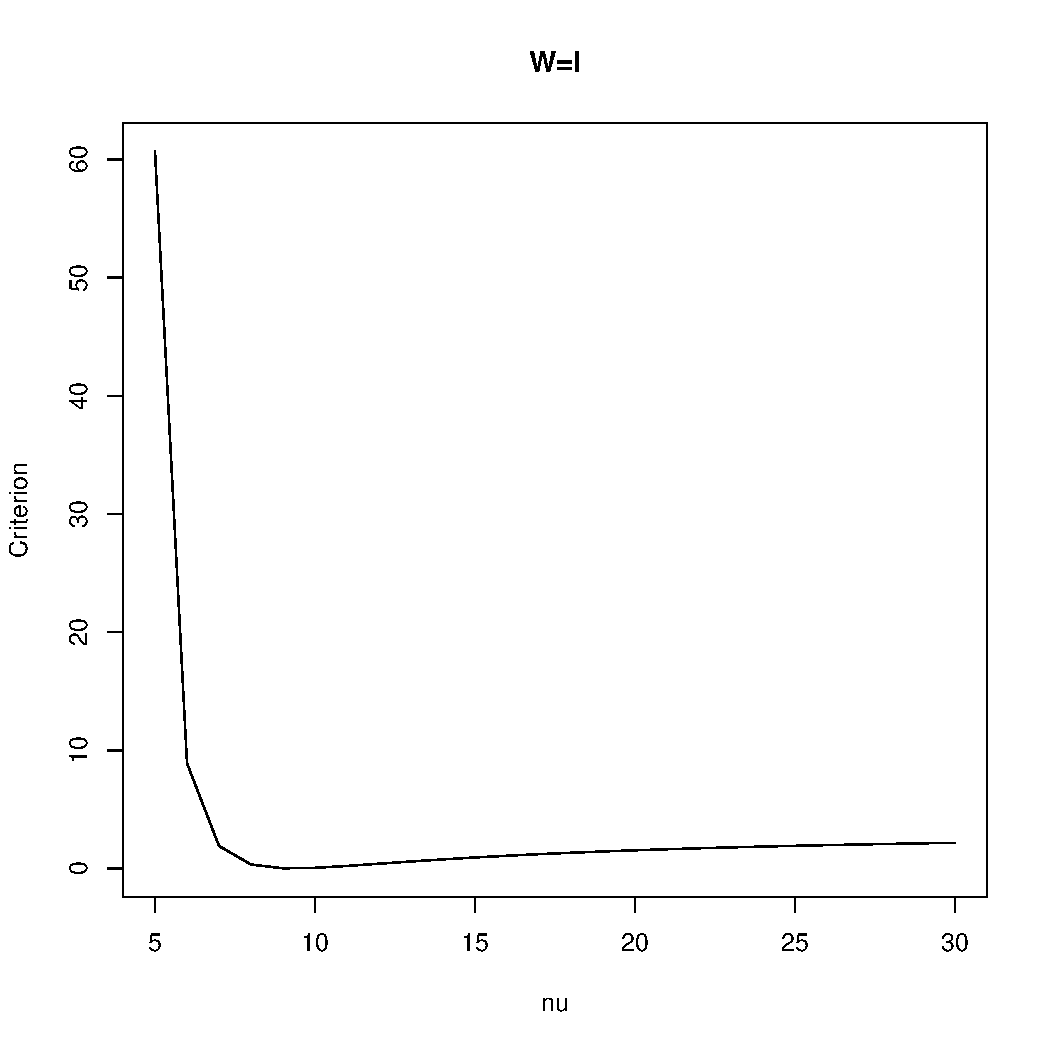
\includegraphics[width=0.7\textwidth]{t-returns_criterion_(W=I).pdf}
    \label{t-returns_criterion_I}
    \caption{Output distribution as a function of the candidates $\nu$ using $W=I$}
    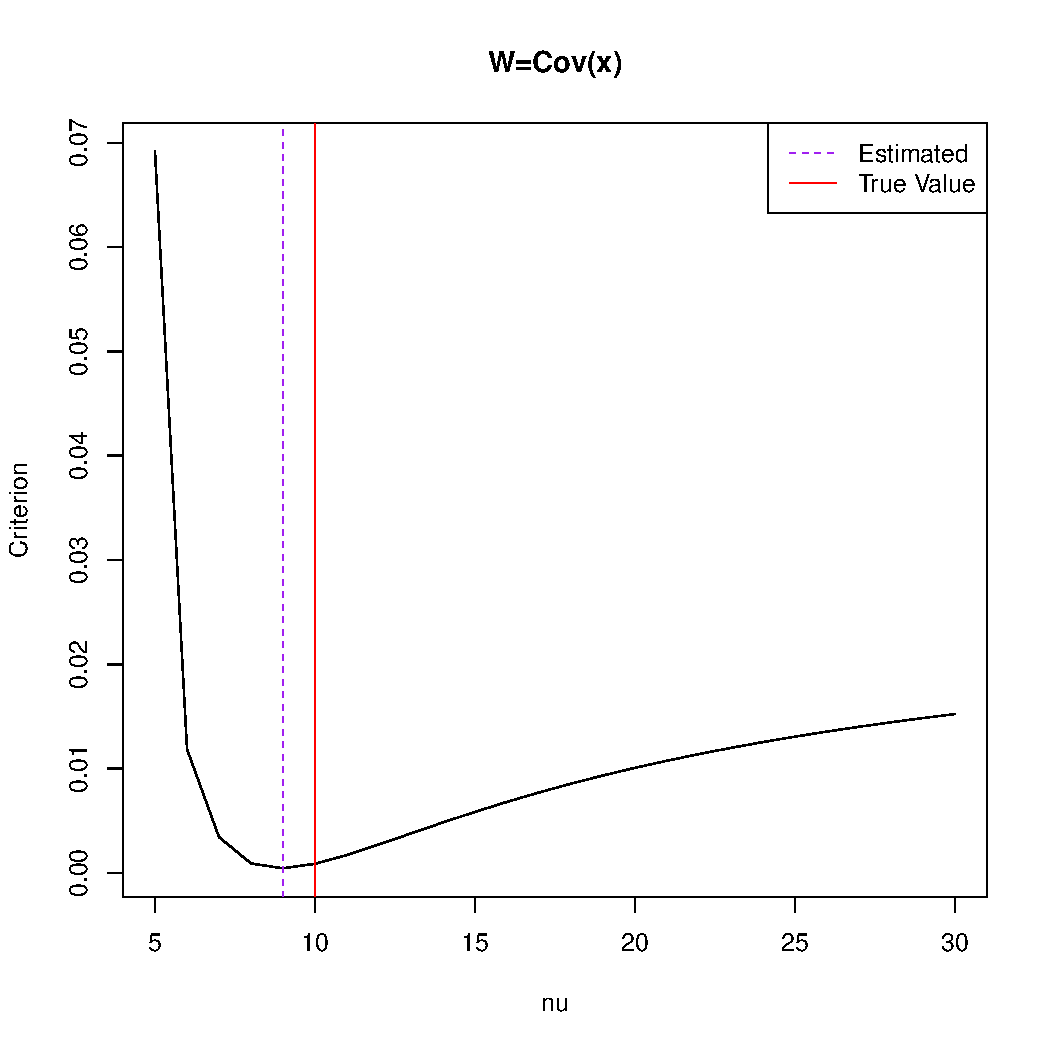
\includegraphics[width=0.7\textwidth]{t-returns_criterion_(W=Sigma^-1).pdf}
    \label{t-returns_criterion_W}
    \caption{Output distribution as a function of the candidates $\nu$ using $W=\Sigma^{-1}$}
\end{figure}


\newpage
As a result, the estimated parameter that minimizes our moment conditions is close to 10. Note that we generated 10000 random returns following a Student distribution with 10 degrees of freedom. Recall the necessary conditions behind the GMM:
\begin{itemize}
    \item Convergence of empirical moments;
    \item Identification;
    \item Asymptotic distribution of empirical moments.
\end{itemize}
With these assumptions it is guaranteed that the estimated GMM parameter converges towards the true parameter. In our case:
\begin{equation*}
        \widehat{\nu}_{GMM} \to \nu_0
\end{equation*}
\begin{equation*}
        \widehat{\nu}_{GMM} \sim N(\nu_0,
        \frac{1}{n}[(\frac{\partial\overline{m}_n\nu_0}{\partial\nu_0^T})^T\Sigma^{-1}\frac{\partial\overline{m}_n\nu_0}{\partial\nu_0^T}]^{-1})
\end{equation*}
The data used in the exercise give an estimated $\nu$ of:
\begin{equation*}
    \begin{cases}
    \widehat{\nu}_{GMM_{1}}=11 \;\;\text{using W=I}\\
    \widehat{\nu}_{GMM_{2}}=9 \;\;\text{using W=}\Sigma^{-1}
\end{cases}
\end{equation*}
Note that the result is not exactly the true value of the parameter but we can converge to the true value by increasing the number of random generated variables, in fact, by the LLN as n increases the GMM estimate converges to the true value, i.e. 10.

Figures \ref{t-returns_density_I} and \ref{t-returns_density_W} show the estimated density functions with $W=I$ and $W=\Sigma^{-1}$ and compares them to a randomly generated (not estimated) t-distribution with 5 degrees of freedom. The Student t-distribution is derived from the normal distribution and as the number of degrees of freedom approaches infinity, the t-distribution tends to the standard normal distribution. In fact, for more than 30 degrees of freedom, the distributions are very close. However, when the number of degrees of freedom is less than 30, the t-distribution has "heavier" tails. In this figure we see that a t-distribution with fewer degrees of freedom (red line, degrees of freedom = 5) has fatter tails than what we have estimated based on our sample with 10 degrees of freedom, regardless of the weighting matrix (black line). 


\begin{figure}
    \centering
    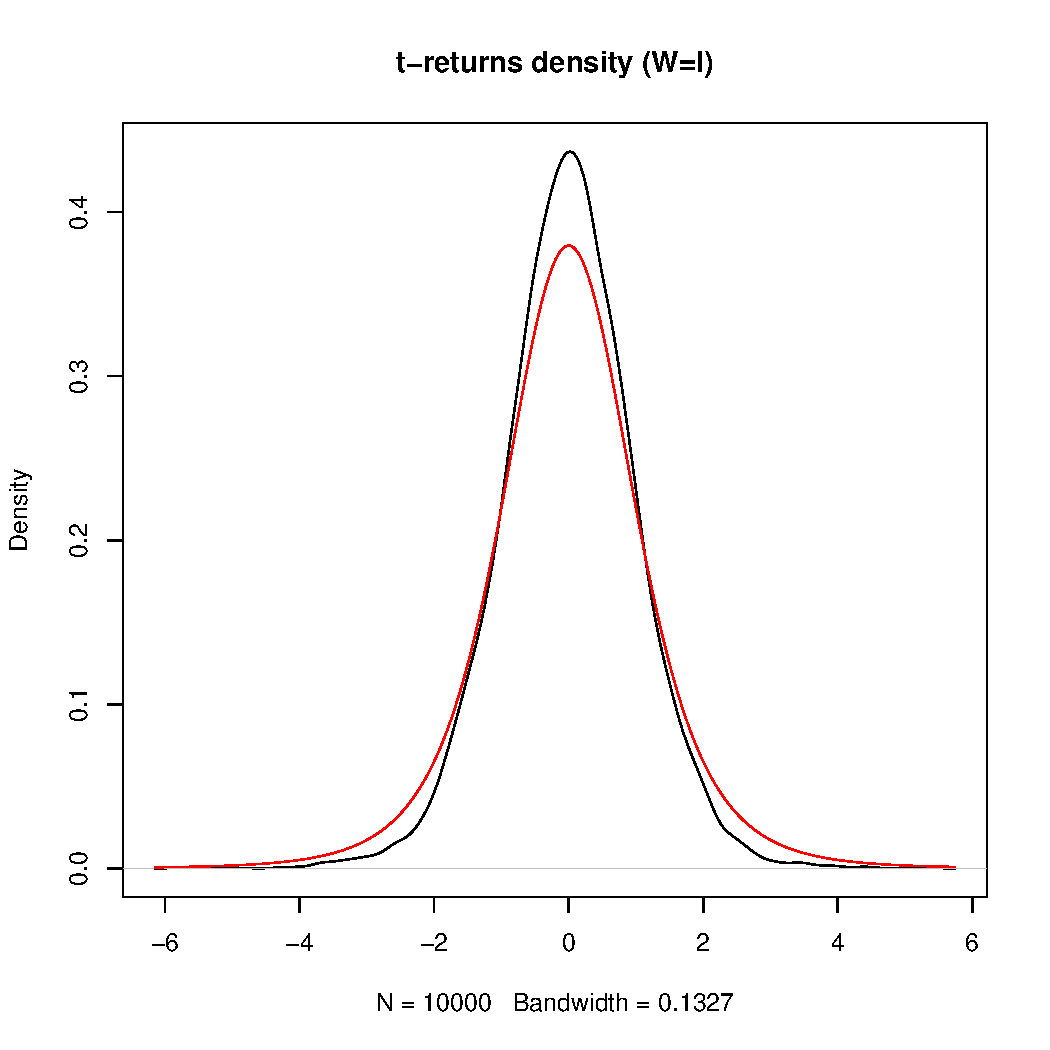
\includegraphics[width=0.7\textwidth]{t-returns_density_(W=I).pdf}
    \label{t-returns_density_I}
    \caption{t-returns density using $W=I$}
    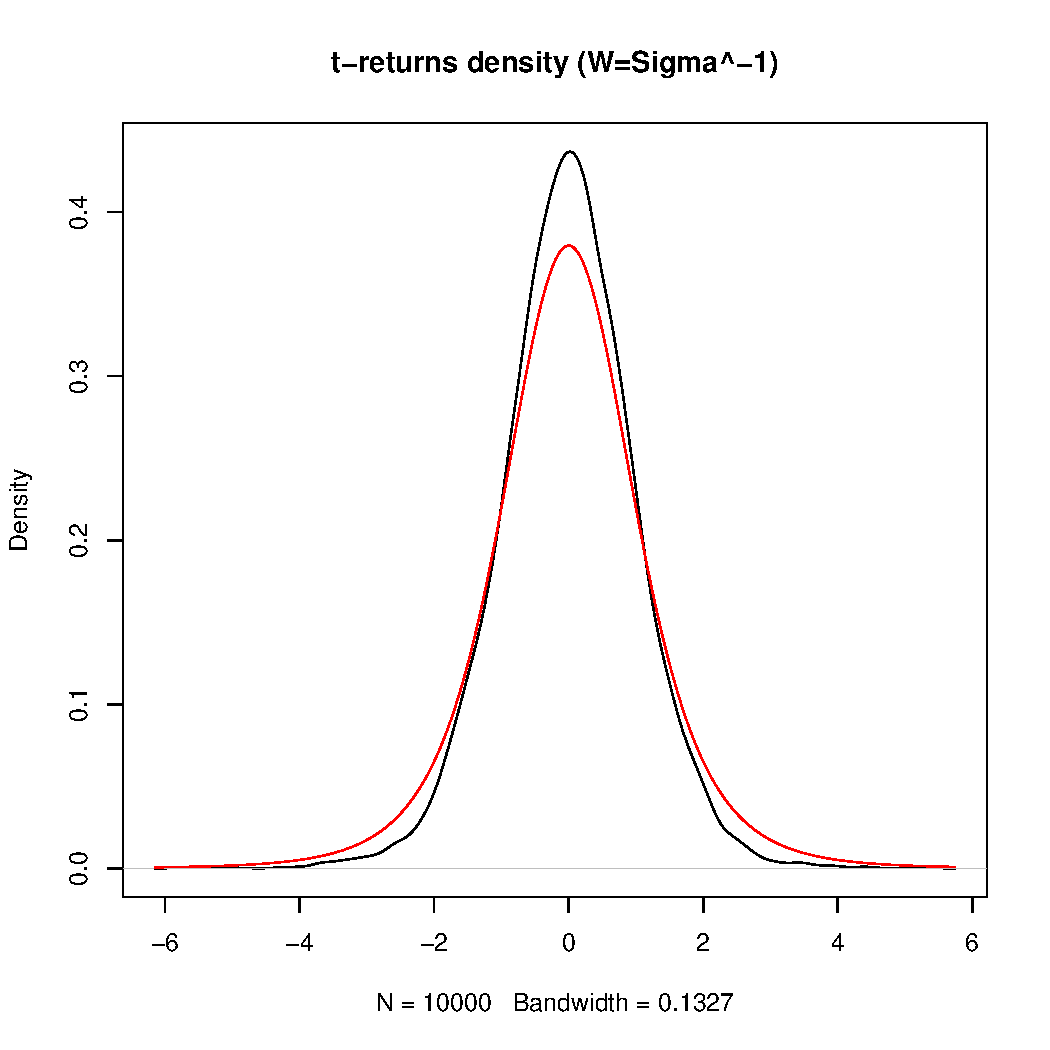
\includegraphics[width=0.7\textwidth]{t-returns_density_(W=Sigma^-1).pdf}
    \label{t-returns_density_W}
    \caption{t-returns density using $W=\Sigma^{-1}$}
\end{figure}
